\newcommand{\PP}{\mathbb{P}}
\newcommand{\EE}{\mathbb{E}}
\newcommand{\One}{\mathds{1}}
\makeatletter
\newcommand*{\rom}[1]{\expandafter\@slowromancap\romannumeral #1@}
\makeatother

\begin{frame}{Outline}
	\tableofcontents[hideallsubsections]
\end{frame}

\section{Introduction}

\begin{frame}{Outline}
	\tableofcontents[current, hideothersubsections]
\end{frame}
\begin{frame}{Motivation}
	\begin{block}{SAGA}
		\begin{itemize}
			\item asdasd
			\item asdasd
			\item asdad
			\item asdasd
		\end{itemize}
	\end{block}
	\pause
	\begin{block}{Challenges}
		\begin{itemize}
			\item \emph{Complex} data
			\item Probabilistic guarantee
			\item Not too optimistic or pessimistic
		\end{itemize}
	\end{block}
\end{frame}

\section{Distributed SAGA}

\begin{frame}{The Proposed Method}
	\centering
	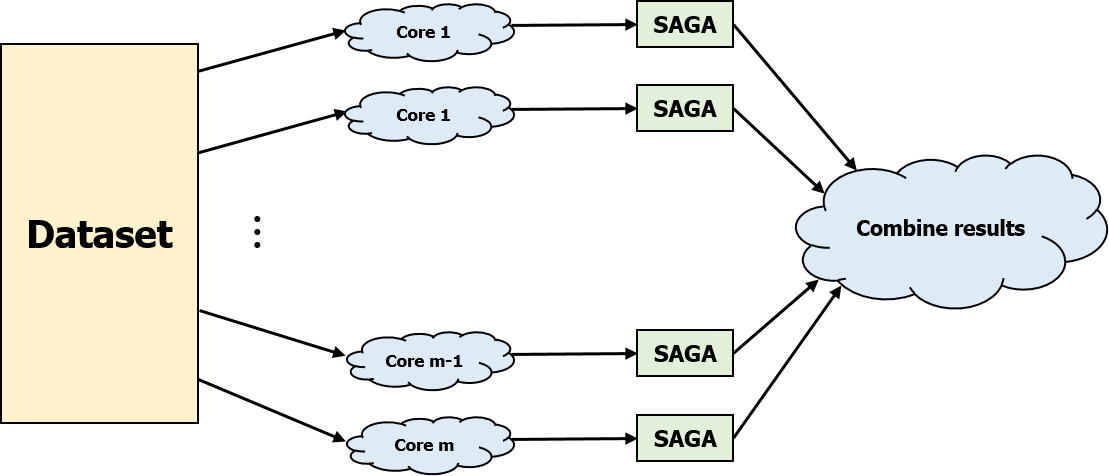
\includegraphics[scale=0.35]{Picture1.PNG}
\end{frame}

\begin{frame}{The Proposed Method}
	\centering
	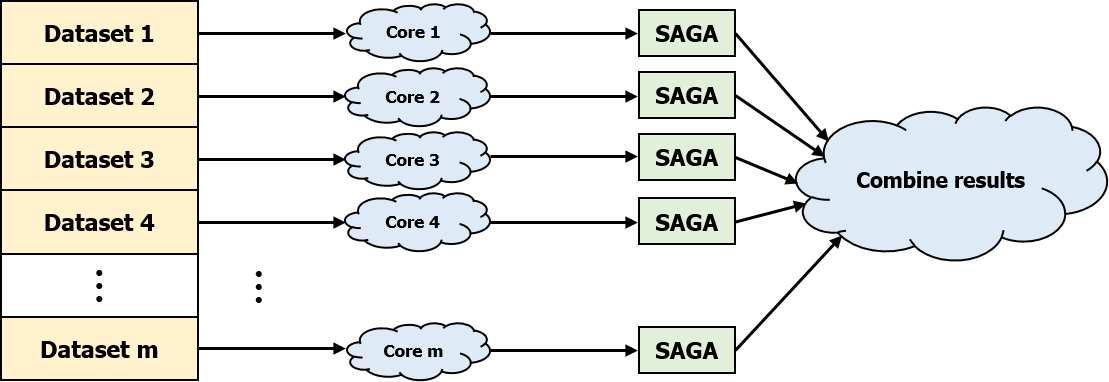
\includegraphics[scale=0.35]{Picture2.PNG}
\end{frame}

